\chapter{2Dアプリケーションの利用}
\label{chapter:2d}

% マルチコンテキストな没入環境において,既存の2Dアプリケーションが利用できることは重要である.

\ref{section:overview:conclusion}で述べたように,
マルチコンテキストな没入環境を社会実装していくうえで,初期の3Dアプリケーションの少なさは
大きな課題となる.
世の中にはすでに有用で,洗練された2Dアプリケーションが数多く存在しており,
アプリケーションそのものだけではなく,ライブラリやデザインシステム,設計パターンなど
多くの知見と資産がある.
既存の2Dアプリケーションがうまく利用できることは,マルチコンテキストな没入環境の発展において
不可欠であり,本システムの重要な設計方針の1つである.

また,\ref{section:intro:problem}や\ref{section:overview:windowing-system}で
言及したとおり,既存の2D Windowing System上で動くアプリケーションは,
他のアプリケーションと連携してマルチコンテキストな2Dデスクトップ環境を実現しており,
マルチコンテキストな没入環境においても,他の2Dアプリケーションや3Dアプリケーションと
連携して利用されることが期待できる.

\section{関連技術・研究}


2Dのウィンドウやディスプレイを没入環境に投影する取り組みはすでに多い.

\ref{section:overview:related-work}で言及したMeta Horizon Workroomsや
Virtual Desktop,Spatialといった商用アプリケーションは,
Microsoft Windows\footnote{Microsoft. ``Meet Windows 11'' \url{https://www.microsoft.com/en-us/windows/windows-11} (accessed 18 Jan, 2023)}
やmacOS\footnote{Apple. ``macOS Ventura'' \url{https://www.apple.com/macos/ventura/} (accessed 18 Jan, 2023)}
といったプロプライエタリなオペレーティングシステムのウィンドウやディスプレイを
没入環境に投影できる(図\ref{fig:share-2d-window}).
これらのアプリケーションはオペレーティングシステムが提供するディスプレイやウィンドウ単位での
画面共有の仕組みを用いて,それをVR空間に投影している.
しかしこの画面共有を用いた手法では,実際の物理ディスプレイの数やサイズ,ウィンドウの配置に
制約をうけたり,本来Windowing Systemが提供するより高度な仕組みを使うことができない.
本来Windowing Systemが提供するより高度な仕組みの例としては,以下のようなものがある.

\begin{itemize}
  \item ウィンドウのコンテンツ(ピクセルマップ)の中で変更があった領域だけを取得し,効率的に
        画面の変更を反映する仕組み
  \item アプリケーション側のアニメーションなどに用いられるリフレッシュレートを制御する仕組み
  \item ポップアップを表示する位置を制御する仕組み
\end{itemize}

\begin{figure}[htbp]
  \centering
  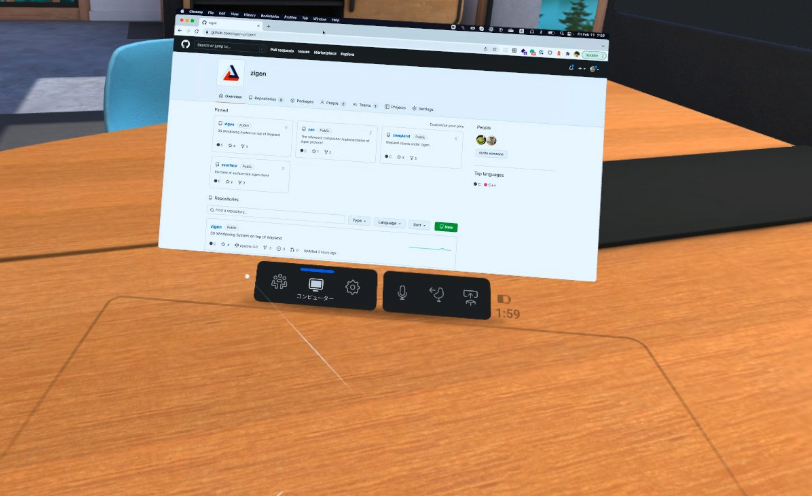
\includegraphics[keepaspectratio, width=0.7\linewidth]{figures/share-2d-window.png}
  \caption{
    Meta Horizon WorkroomsでのPC画面の共有機能.
  }
  \label{fig:share-2d-window}
\end{figure}

これに対して,Reiling\cite{reiling}が提案した没入環境向けのコンポジッタでは,
既存の2D Windowing Systemのプロトコルも実装することで,没入環境で既存の2Dアプリケーションが
利用できるようにした(図\ref{fig:reiling-2d}).

\begin{figure}[htbp]
  \centering
  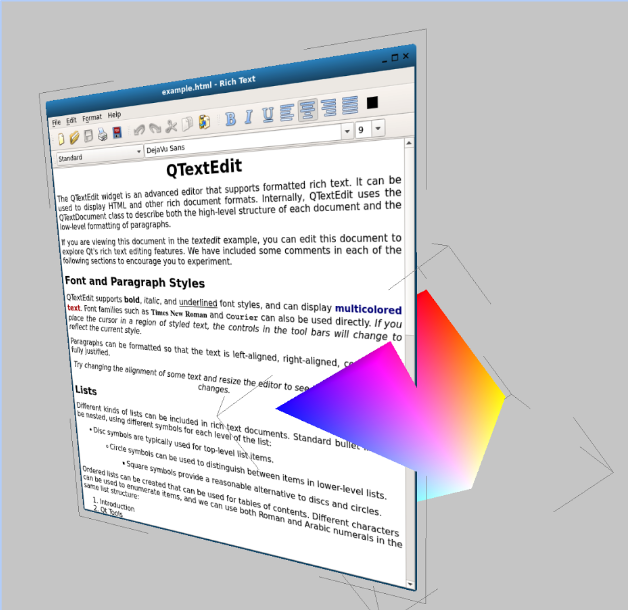
\includegraphics[keepaspectratio, width=0.7\linewidth]{figures/reiling-2d.png}
  \caption{
    motorcar\cite{reiling}での既存の2Dアプリケーションの表示.
    (Adapted from Reiling. ``Defense Slides''(Google Slide) \url{https://docs.google.com/presentation/d/1svgGMxxbfmcHy_KuS5Q9hah8PQOsXqvjBKOoMIzW24Y/edit?usp=sharing} (accessed 18 Jan, 2023))
  }
  \label{fig:reiling-2d}
\end{figure}

この手法では,コンポジッタが2Dアプリケーションと直接やり取りするため,
既存の2Dアプリケーションを改変しないという制約のもとで,
2Dアプリケーションの表示や操作に関して最大限の自由度がある.

しかし,Reilingの提案では,3Dアプリケーションを2Dアプリケーションと連携して使うための
工夫については言及がなかった.3Dアプリケーションと2Dアプリケーションとを連携して使うためには
3Dアプリケーションのプロトコルの設計も工夫する必要がある.

% 2Dアプリケーションと3Dアプリケーション間のドラッグ \& ドロップ
% といった連携を実現してはいなかった.

% Workroomsのような画面共有ベースのプロダクト
% * ホストのWindowing Systemが提供しているAPIに制約をうけ、Dndなどは実現できない。
% Forrestも入れて良いかと思う。

\section{提案手法}

% 本システムでは,3Dアプリケーションに対する操作に関するプロトコルを既存の2DのWindowing System
% と変換可能な形に設計することで,3Dアプリケーションと既存の2Dアプリケーション間の
% ドラッグ \& ドロップを可能にした.

% 2DのWindowing Systemのプロトコルと変換可能な操作に関するプロトコルを設計するうえで,
% 本システムでは始点と方向をもつRayを用いてアプリケーションに操作を与えることにした.
% Rayによる操作は没入環境では一般的だが,特に本システムではRayを定義することで,
% RayとWindowが交差した位置にカーソルを定義でき,
% これを用いてRayとカーソルを変換できるので重要である.

% 2D Windowing Systemにおけるドラッグ \& ドロップのプロトコルは
% イベント(コンポジッタからアプリケーションへの通信)と
% リクエスト(アプリケーションからコンポジッタへの通信)の複雑な組み合わせで実現されており,
% ドラッグ \& ドロップの開始のリクエスト,
% データを送る側がどのような形式のデータで送ることができるかの候補(mime-type)を提示するリクエスト,
% 送る側のアクションの意図(データのコピーなのか,移動なのか)を提示するリクエスト,
% ドラッグ中のカーソルの位置を知らせるイベント,など20種類以上存在する.

% 本システムではこのドラッグ \& ドロップのプロトコルのうち,カーソルに関する部分を
% Rayに置き換えたプロトコルを3Dアプリケーション用に定義した.
% そして,3Dコンポジッタと既存の2Dアプリケーションとの間に,Rayの動きを
% Window上のカーソルの動きに変換するコンポーネントを入れることで,
% 3Dアプリケーションと2Dアプリケーション間のドラッグ \& ドロップを実現した(図\ref{fig:dnd-architecture}).

% もっと全体的に変換可能に設計しました。フレームとか、Rayそのものとかも
% その結果、Dndもできるようになりました。の方がいいか。

本システムでは,3Dアプリケーションに対する操作に関するプロトコルを,
既存の2DのWindowing Systemと変換可能な形に設計することで,
2Dアプリケーションを3Dアプリケーションとより連携して使えるようにした.

2DのWindowing Systemではカーソルを介してそれぞれのアプリケーションに操作を加えるが,
本システムでは始点と方向ベクトルを持つRayを介してアプリケーションに操作を与えることにした.
Rayによる操作は没入環境では一般的だが,特に本システムではRayを定義することで,
Rayとウィンドウが交差した位置にカーソルを定義でき,これを用いてRayの操作をカーソルの操作に変換できるため重要である.

本システムでは2DのWindowing Systemの操作に関するプロトコルのうち,カーソルに関する部分だけを
Rayに置き換えたプロトコルを3Dアプリケーションの操作のために定義した.
そして,3Dコンポジッタと既存の2Dアプリケーションとの間にRayの動きをウィンドウ上のカーソルの
動きに変換するコンポーネントを入れた(図\ref{fig:dnd-architecture}).
このコンポーネントの主な役割は没入環境の3D空間上にウィンドウを表す長方形の領域を定義し,
既存の2D Windowing Systemのコンポジッタとして振る舞うことで,
既存の2Dアプリケーションから描画内容を受け取り,それを長方形領域に描画すると同時に,
Rayとその長方形領域とが重なった位置にカーソルを定義して,Rayの操作をカーソルの操作に変換して
アプリケーションに伝えることである.
その他にも2D Windowing Systemのコンポジッタとしてアプリケーションとやりとりすべき内容
(フレーム同期・ウィンドウの移動やリサイズのリクエストの処理など)を実装している.

これによって,2Dアプリケーションと3Dアプリケーションを同じデバイスで,同じRayを介して
操作できるようになる.
また,本システムではドラッグ \& ドロップに関するプロトコルもRayを用いて再定義している.
2D Windowing Systemにおけるドラッグ \& ドロップのプロトコルは
イベント(コンポジッタからアプリケーションへの通信)と
リクエスト(アプリケーションからコンポジッタへの通信)の複雑な組み合わせで実現されており,
ドラッグ \& ドロップの開始のリクエスト,
データを送る側がどのような形式のデータで送ることができるかの候補(mime-type)を提示するリクエスト,
送る側のアクションの意図(データのコピーなのか,移動なのか)を提示するリクエスト,
ドラッグ中のカーソルの位置を知らせるイベント,など20種類以上存在する.
これらを全て3Dアプリケーション用に定義し直すことで,本システムでは既存の2Dアプリケーションと
3Dアプリケーション間でのドラッグ \& ドロップを実現しており,
これはまさに本システムでしか実現できない特徴である.


\begin{figure}[htbp]
  \centering
  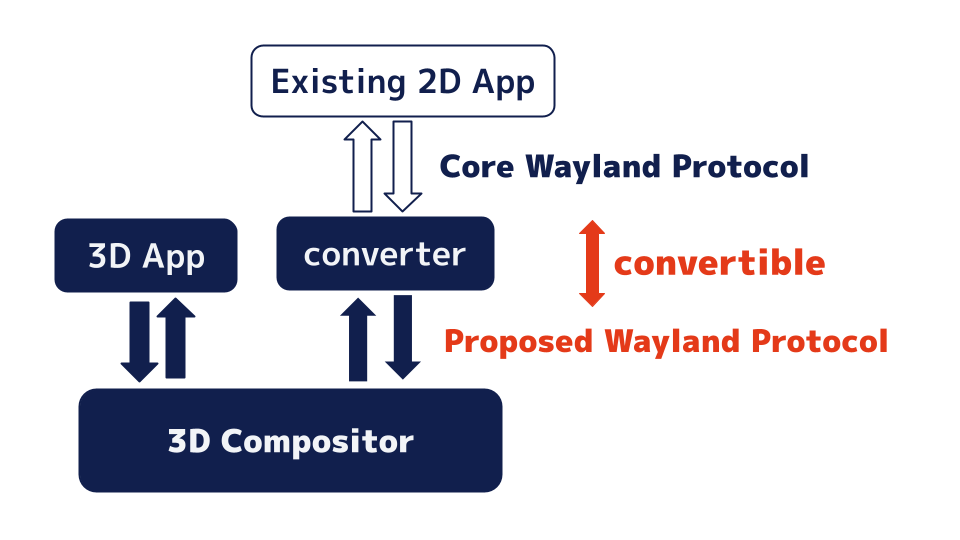
\includegraphics[keepaspectratio, width=0.9\linewidth]{figures/dnd-architecture.png}
  \caption{
    本システムでの既存の2Dアプリケーションを利用する仕組み.
  }
  \label{fig:dnd-architecture}
\end{figure}

\section{評価}

本システムにおいて2Dアプリケーションに関する設計が有効であることを確かめるために,
サンプルのアプリケーションを用意した(図\ref{fig:dnd-apps}).
1つは改変のない既存の2Dブラウザ
(Google Chrome\footnote{Google. ``Google Chrome'' \url{https://www.google.com/chrome/} (accessed 18 Jan, 2023)}
図\ref{fig:dnd-apps}右側),
もう1つは地球などの天体を表示する3Dアプリケーション(図\ref{fig:dnd-apps}左側)である.
また今回はRayの操作にはマウスを用い,マウスの2次元の移動量をRayの方向ベクトルの変化にマッピングした.

\begin{figure}[htbp]
  \centering
  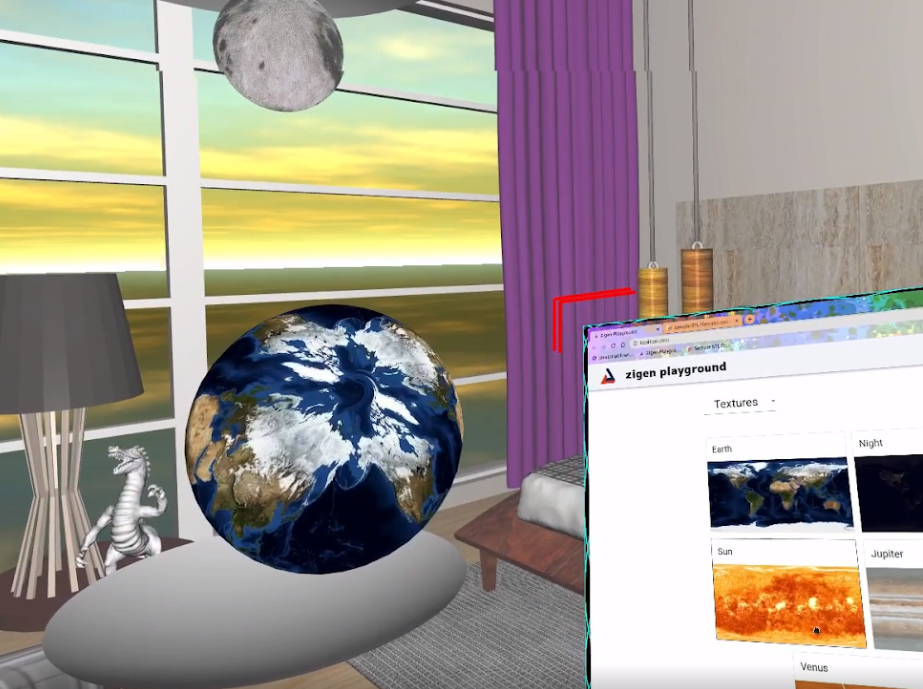
\includegraphics[keepaspectratio, width=0.9\linewidth]{figures/dnd-apps.png}
  \caption{
    サンプルの3DアプリケーションとGoogle Chrome
  }
  \label{fig:dnd-apps}
\end{figure}

まず,このRayを用いてブラウザに対してカーソルの移動,クリック,スクロールの基本的な操作が
可能であることを確かめた.
また天体のアプリケーションに本システムで定義したドラッグ \& ドロップのプロトコルを実装し,
ブラウザからのドラッグ \& ドロップによって天体のテクスチャデータを
更新できることを確かめた(図\ref{fig:dnd}).

\begin{figure}[htbp]
  \centering
  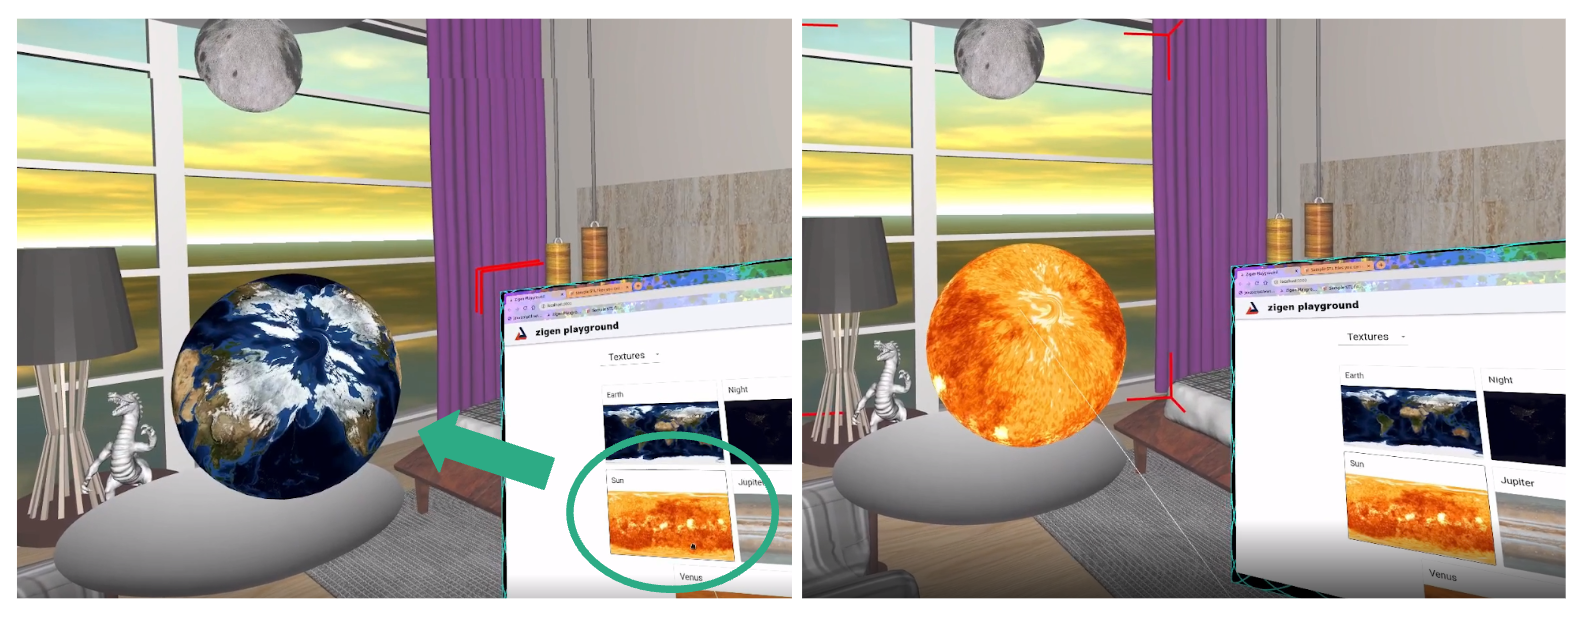
\includegraphics[keepaspectratio, width=\linewidth]{figures/dnd.png}
  \caption{
    3Dアプリケーションと2Dアプリケーションとの間でドラッグ \& ドロップする様子.
    左図がドラッグ \& ドロップの前で,ブラウザから太陽のテクスチャを
    ドラッグ \& ドロップすることで,右図のように地球のテクスチャを太陽に変化させることができた.
  }
  \label{fig:dnd}
\end{figure}

% 2D のダメージを使える。
% 物理ディスプレイの枚数や、サイズの制約を受けない
% Dnd ができたということ。
% 汎用性に欠ける

\section{まとめ}

既存手法では2Dアプリケーションを3Dアプリケーションと同時に没入環境に提示することは実現していたが,
3Dアプリケーションと2Dアプリケーションとの協調の可能性までは検討されていなかった.
本システムでは3Dアプリケーションの操作に関するプロトコルを2Dアプリケーションの
操作に関するプロトコルと変換可能な形に,丁寧に設計することで,2Dアプリケーションと
3Dアプリケーションとの間のドラッグ \& ドロップのような協調が可能であることを示した.

本システムではRayを用いて2D・3D両方のアプリケーションを操作するが,
どのようなハードウェアでこのRayを操作するかまでは規定しなかった.
これは様々なハードウェアがシステムと連結できるようにするためだが,
2Dアプリケーションと3Dアプリケーションの両方に対して操作しやすい
デバイスに関しては研究の余地があり,今後の研究課題としたい.
